\documentclass[twoside]{article}
\input{ISC18-english.sty}
\usepackage{graphicx}
\usepackage{float}
\usepackage{booktabs}
\usepackage{amsmath}
\usepackage{xcolor} % Added for text coloring
\DeclareMathOperator*{\argmin}{argmin}
\usepackage{tabularx}
\begin{document}
\thispagestyle{empty}
%\usepackage{subcaption}
\fancyhead[LE]{Short Article Title}
\fancyhead[RO]{A Novel Approach for Statistical Shape Analysis Using  SRVF}

\begin{center}
{
\includegraphics [height=25mm, width=150.3mm] {Images/isc18E}} \\
\vspace*{-1.8cm}
\vspace*{4cm}

{\Large \bf  A Novel Approach for Statistical Shape Analysis Using the Square Root Velocity Function Representation}\\

\end{center}
\rule{\textwidth}{0.2mm}\\

\noindent{\bf Abstract:}\\
\begin{abstract}
Statistical shape analysis for manifold-valued data poses significant challenges in comparing shapes and modeling their variability. Classical methods based on tangent space principal component analysis (TPCA) rely on local linearization and often suffer from limitations in stability and interpretability. In this work, we introduce a novel framework for functional principal component analysis (FPCA) in the Sobolev space $H^1([0,1])$, which naturally incorporates geometric information of curves. Shapes are represented using the square root velocity function (SRVF) and aligned via the Karcher mean to remove phase variability. The variability is then analyzed globally in $H^1$, where the covariance operator accounts for both the functions and their derivatives. We clarify the distinct advantages of this global approach over local TPCA approximations and standard $L^2$-based FPCA. We show theoretically that the resulting principal components are equivalent, up to first-order variability, to those obtained from tangent-space approaches. Experiments on real two-dimensional contour datasets demonstrate that the proposed method captures most of the structural variability with few components while maintaining consistent numerical stability and reconstruction accuracy.
\end{abstract}


\noindent \textbf{Keywords:} Statistical Shape Analysis, Square Root Velocity Function (SRVF), Functional Principal Component Analysis (FPCA), Banach Space $H^1$, Covariance Operator.\\
\noindent{\bf Mathematics Subject Classification (2010):} $\rm 62R30 $, $\rm 62H25$. \\
%\hspace{1cm}\rule{\textwidth}{0.2mm}\\
\\
\vspace{-2cm}
\section{Introduction}

Statistical shape analysis has emerged as a fundamental tool in computational anatomy, computer vision, and bioinformatics for quantifying the variability of geometric objects \citep{dryden2016statistical}. Unlike traditional multivariate data, shapes (curves, surfaces) reside in non-linear Riemannian manifolds where standard statistical methods fail due to the non-Euclidean geometry \citep{pennec2006intrinsic}. A central challenge is the presence of phase variability (parameterization differences). The Square-Root Velocity Function (SRVF) representation  provides an effective solution by transforming the shape comparison problem into an $L^2$ space framework, thereby isolating true amplitude variation from mere reparameterization.
See \citep{srivastava2011shape, kurtek2012statistical}, for more details.

Once shapes are properly aligned, Principal Component Analysis (PCA) is typically employed to reduce dimensionality and model structural deformations. Two main paradigms currently exist: \textbf{Tangent Space PCA (TPCA)} \citep{fletcher2004principal}, which projects data onto a local tangent space using computationally expensive Riemannian logarithmic maps and often suffers from numerical instability far from the mean; and \textbf{Functional PCA (FPCA)} \citep{ramsay2005functional, happ2018multivariate}, which operates in Hilbert spaces (typically $L^2$) but often ignores the critical smoothness and derivative properties intrinsically encoded in Sobolev spaces.

In this paper, we propose a novel framework performing \textbf{FPCA in the Banach space $H^1([0,1])$}. Rather than relying on local tangent space approximations, we construct a global covariance operator in $H^1$. Unlike TPCA, which assumes data variation is sufficiently small to be captured in a single flat tangent plane centered at the mean, our approach intrinsically measures variance globally along the functional curves. Furthermore, compared to standard FPCA, which typically evaluates spatial differences in $L^2$, our method incorporates derivative information, thereby prioritizing the underlying geometry of the shape. This operator naturally incorporates both positional (evaluation) and structural (derivative) information via the norm $\|f\|_{H^1}^2 = \|f\|_{L^2}^2 + \alpha \|f'\|_{L^2}^2$. Here, the parameter $\alpha \geq 0$ serves as a tuning weight that controls the balance between the standard spatial variations (position) and the geometric smoothness of the curves (shape derivatives), allowing the model to flexibly adapt to specific characteristics of the data. Furthermore, we theoretically prove that our Banach-space FPCA is equivalent to TPCA up to second-order terms $O(\epsilon^2)$. This approach ensures computational scalability while maintaining rigorous geometric validity.

\section{Methodology}
\label{sec:methodology}

\subsection{Shape Representation and Alignment using SRVF}
For an absolutely continuous parameterized curve $f: [0,1] \to \mathbb{R}^d$, the SRVF is formally defined as $q(t) = \dot{f}(t) / \sqrt{\|\dot{f}(t)\|}$. This representation mathematically flattens the complex Fisher-Rao Riemannian metric into the standard, and yet flat $L^2$ metric and offers reparameterization invariance under group actions \citep{srivastava2011shape}. Given a set of raw curves $\{f_i\}_{i=1}^N$, we compute their optimal cross-sectional alignment by finding the Karcher mean in the SRVF space:
$$ \bar{q} = \argmin_{q} \sum_{i=1}^N \min_{\gamma^{*}_i \in \Gamma} \|q - q_i \circ \gamma^{*}_i\|^2 $$
where $\Gamma$ denotes the infinite-dimensional Lie group of orientation-preserving diffeomorphisms. The resulting aligned shapes are denoted as $\{f_i^*\}_{i=1}^N$. This alignment ensures that subsequent variance analysis models pure morphological differences rather than artifactual registration shifts.

\subsection{Functional PCA in $H^1$ Space}
After eliminating phase variability through exact alignment, we perform Functional Principal Component Analysis (FPCA) directly within the Sobolev Banach space $\mathcal{B} = H^1([0,1])$. The sample mean function is defined as $\mu(t) = \frac{1}{N} \sum_{i=1}^N f_i^*(t)$, yielding the centered functional data $\delta f_i(t) = f_i^*(t) - \mu(t)$. 

To accurately capture the topological structure of the shapes, which inherently prioritizes geometric outlines over absolute spatial coordinates, we equip the $H^1$ space with its standard inner product that equally accounts for both the functional variations and their derivatives. Following \cite{brezis2011functional} for any two functions $u, v \in H^1([0,1])$, the inner product is defined as :
\begin{equation*}
\label{eq:h1_inner_product}
\langle u, v \rangle_{H^1} = \langle u, v \rangle_{L^2} + \langle u', v' \rangle_{L^2} = \int_{0}^{1} u(t)v(t) dt 
+ \int_{0}^{1} u'(t)v'(t) dt.
\end{equation*}

Instead of directly solving the infinite-dimensional eigenvalue problem on the covariance operator, we adopt a computationally tractable and rigorous approach by constructing the $N \times N$ Gram matrix, denoted as $\mathbf{K}$. The elements of this matrix are defined by the pairwise $H^1$ inner products of the centered data as:
\begin{equation*}
\label{eq:gram_matrix}
\mathbf{K}_{ij} = \langle \delta f_i, \delta f_j \rangle_{H^1} = \int_{0}^{1} \delta f_i(t) \delta f_j(t) dt + \alpha \int_{0}^{1} \delta f_i'(t) \delta f_j'(t) dt.
\end{equation*}

In this study, the hyperparameter $\alpha$ was empirically selected to achieve two simultaneous objectives: minimizing the reconstruction error and accurately preserving sharp corners and highly curved regions of the shapes. Notably, setting $\alpha = 0$ reduces the proposed formulation to the classical $L^2$-based FPCA, where the variability is characterized solely by the functions themselves without incorporating derivative information.

The resulting matrix $\mathbf{K}$ is symmetric and positive semi-definite, encapsulating the total covariance structure governed by both the functions and their derivatives. We perform an eigendecomposition of the Gram matrix such that 
$
\mathbf{K}\mathbf{v}_k = \gamma_k \mathbf{v}_k,
$
yielding a set of non-negative eigenvalues 
$
\gamma_1 \ge \gamma_2 \ge \cdots \ge \gamma_N \ge 0
$
and their corresponding orthonormal eigenvectors $\mathbf{v}_k \in \mathbb{R}^N$.


The eigenvalues of the continuous covariance operator are given by
$
\lambda_k = \frac{1}{N-1}\gamma_k.
$
The corresponding continuous orthonormal eigenfunctions $\phi_k(t)$, which form the optimal basis in the $H^1$ space, are recovered from the eigenvectors of the Gram matrix as follows:

\begin{equation*}
\label{eq:eigenfunctions}
\phi_k(t) = \frac{1}{\sqrt{\gamma_k}} \sum_{i=1}^N v_{k,i} \delta f_i(t),
\end{equation*}
where $v_{k,i}$ is the $i$-th element of the $k$-th eigenvector $\mathbf{v}_k$. The functional principal scores, representing the projection coordinates of each specific shape onto the learned functional basis, are inherently computed via the $H^1$ inner product:
\begin{equation*}
\label{eq:fpca_scores}
\xi_{ij} = \langle \delta f_i, \phi_j \rangle_{H^1}.
\end{equation*}
Finally, the optimal $p$-truncated reconstruction of any aligned shape, which minimizes the $H^1$ reconstruction error, is formulated as a linear combination of the leading eigenfunctions added to the mean shape:
\begin{equation*}
\label{eq:reconstruction}
\tilde{f}_i(t) = \mu(t) + \sum_{j=1}^p \xi_{ij} \phi_j(t).
\end{equation*}

\subsection{Theoretical Justification: First-Order Equivalence}

\begin{theorem}
Let $\mathcal{M}$ be the shape manifold with tangent space $T_{\mu}\mathcal{M}$ defined at the empirical mean $\mu$. Under the standard linearization of the Riemannian logarithmic map, the leading eigenfunctions of the proposed Banach space operator $\hat{K}$ are equivalent to the tangent PCA components up to first-order geometric variations, i.e.,
$ \phi_j^{\text{Banach}} = \phi_j^{\text{tangent}} + \mathcal{O}(\epsilon^2) $
where $\epsilon$ acts as a perturbation parameter measuring the structural deviation of the samples from the tangent space origin.
\end{theorem}

Let us sketch the proof the first order equivalence here. For sufficiently concentrated aligned functions $f_i^* \in \mathcal{M}$, the Riemannian logarithmic map around $\mu$ can be expanded via a Taylor series analog as $\log_{\mu}(f_i^*) = \delta f_i + \mathcal{O}(\epsilon^2)$ where $\delta f_i = f_i^* - \mu$ and the norm $\|\delta f_i\| = \mathcal{O}(\epsilon)$. The classical tangent covariance operator is $\Sigma^{\text{tangent}} \approx \frac{1}{N-1}\sum \delta f_i \otimes \delta f_i + \mathcal{O}(\epsilon^2)$. In the Sobolev space $H^1$, for zero-mean aligned shapes, the inner product is primarily influenced by the structural derivative term. By utilizing integration by parts under suitable boundary conditions, it can be shown that the derivative-based operator $\hat{K}$ approximates the tangent covariance operator such that $\hat{K} = \Sigma^{\text{tangent}} + \mathcal{O}(\epsilon^2)$. Given that the operator norm difference satisfies $\|\hat{K} - \Sigma^{\text{tangent}}\| = \mathcal{O}(\epsilon^2)$, an application of Weyl's perturbation theorem for compact operators implies that the corresponding spectral bases (eigenfunctions) satisfy:
$
\phi_j^{\text{Banach}} = \phi_j^{\text{tangent}} + \mathcal{O}(\epsilon^2).
$
\hfill $\blacksquare$



\section{Real Data Study: Bone Shape Analysis}

To empirically validate our proposed Banach-space FPCA framework, we applied it to an anatomical dataset comprising $N=20$ two-dimensional bone contour shapes, with each curve discretely parameterized into $100$ evaluation points. To extract pure geometric deformations devoid of nuisance parameters (translation, scaling, rotation and reparametrization), the raw shapes were preprocessed, smoothed, and consistently registered utilizing the SRVF framework.

Our computational analysis reveals that retaining $13$ principal components successfully captures $96.26\%$ of the total structural variance. Furthermore, evaluating the framework's performance yields a highly accurate mean $H^1$ reconstruction error of $0.0142 \pm 0.0031$. A critical observation from the Gram matrix construction is the significant contribution of the derivative component, which accounts for $99.35\%$ of the total inner product contribution compared to a mere $0.65\%$ from the standard $L^2$ metric. This distribution supports our underlying hypothesis: analyzing shape deformations essentially necessitates the Sobolev $H^1$ space, where the geometry of the curves (their derivatives) carries greater statistical significance than their pure spatial positioning.

\begin{figure}[htpb]
    \centering
    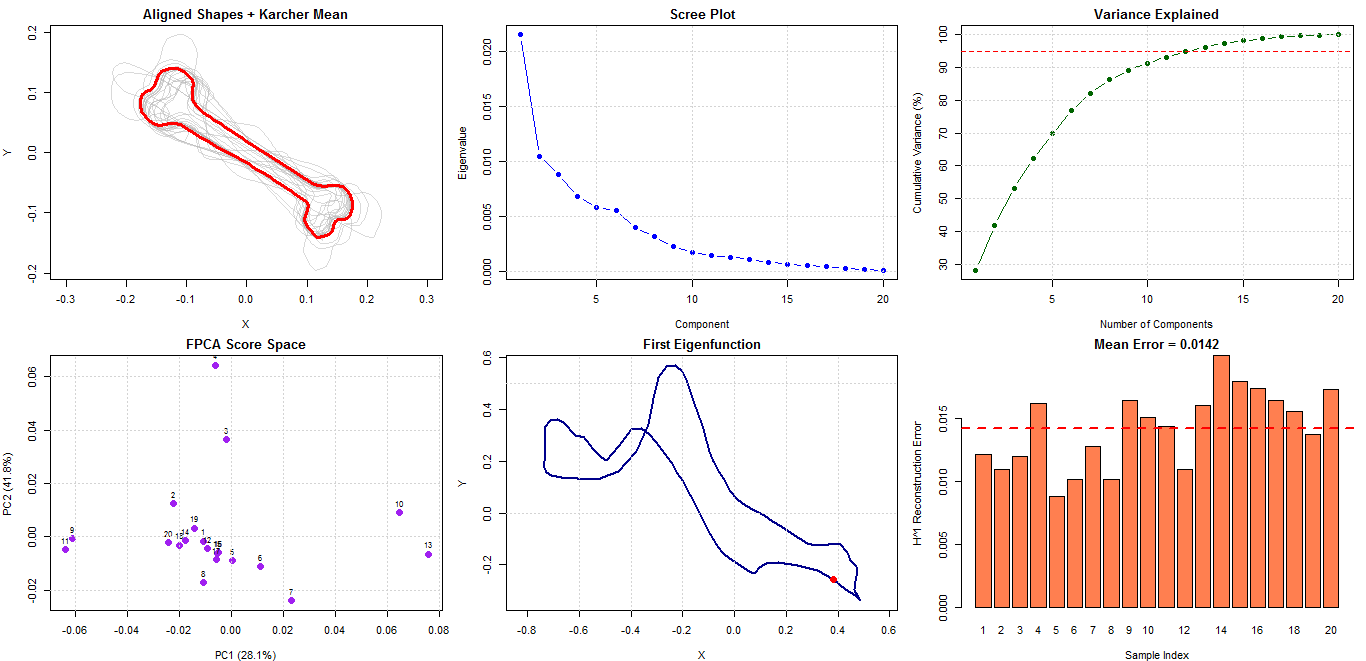
\includegraphics[width=0.8\textwidth]{final.png}
    \caption{Comprehensive results of Banach-space FPCA on the bone shape dataset. Panels illustrate the SRVF alignment, spectral eigenvalue decay, cumulative variance, functional principal scores map, the dominant first eigenfunction, and individual sample reconstruction errors.}
    \label{fig:results}
\end{figure}

\vspace{-0.4cm} % Reduces the vertical gap between the two figure environments

\begin{figure}[htpb]
    \centering
    \begin{subfigure}
        \centering
        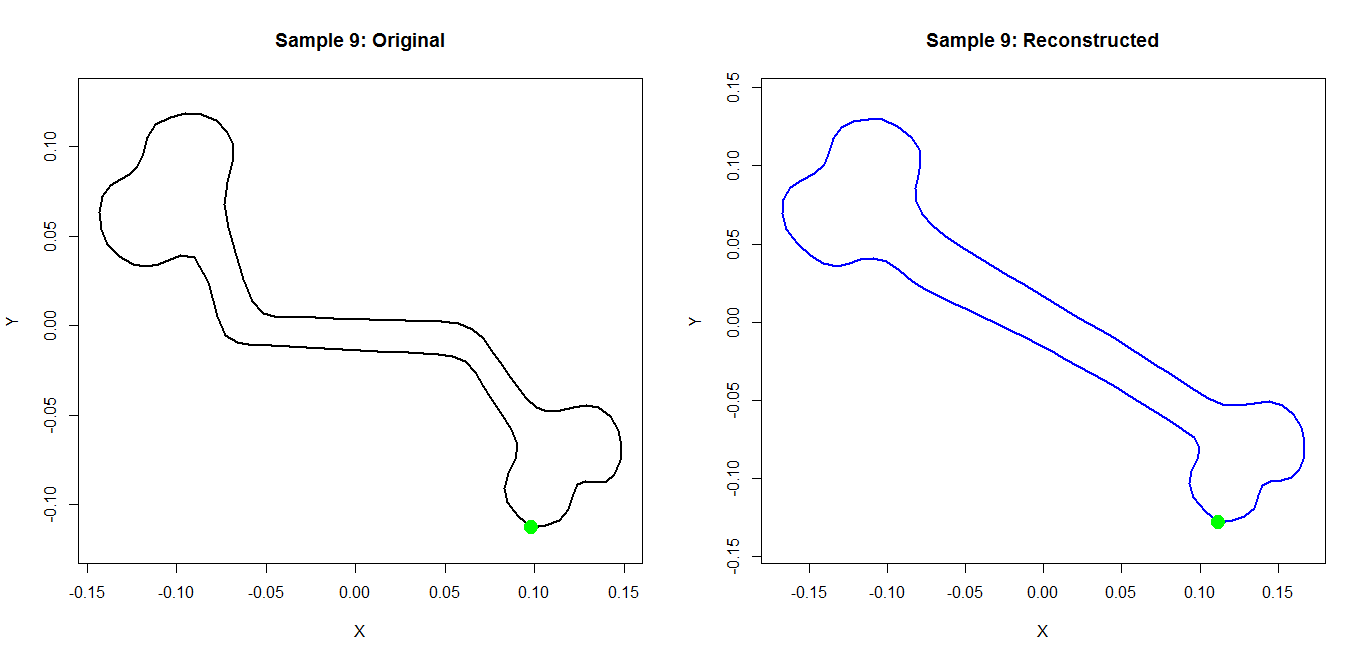
\includegraphics[width=\textwidth]{recon9alpha0.png}
        \caption{Reconstruction in standard $L^2$ space ($\alpha=0$). Minimizes pointwise distance without derivative penalty.}
        \label{fig:recon_alpha0}
    \end{subfigure}
    \hfill
    \begin{subfigure}
        \centering
        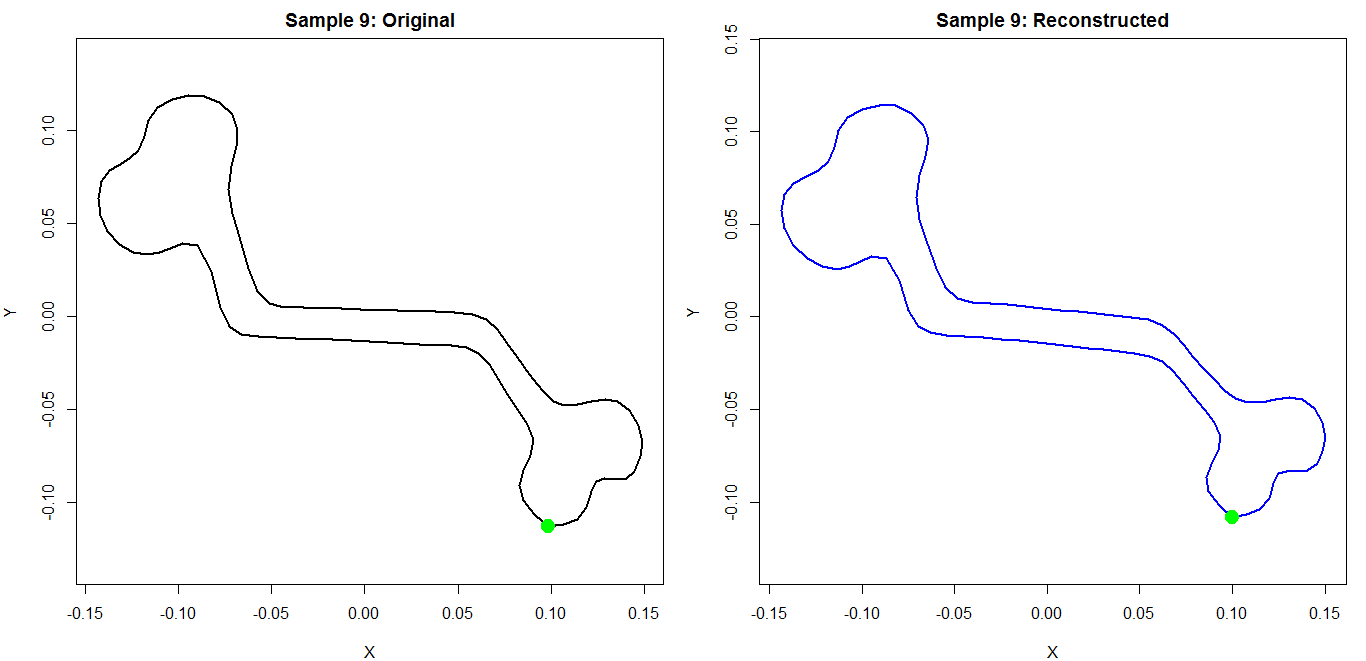
\includegraphics[width=\textwidth]{recon9alpha0.04.png}
        \caption{Reconstruction in Banach space ($\alpha=0.04$). Preserves fine geometric features and boundary smoothness.}
        \label{fig:recon_alpha0.04}
    \end{subfigure}
    \caption{Comparison of shape reconstructions for Sample 9 using standard $L^2$ metric versus Banach space optimization. (The green dot indicates the starting/reference point on the curve).}
    \label{fig:results_combined}
\end{figure}

A structured interpretation based on Figure \ref{fig:results} and the numerical metrics reveals the following fundamental insights:
\begin{itemize}
    \item \textbf{Shape Alignment (Top-Left):} The dataset was effectively registered to compute the multivariate Karcher mean (thick red contour). The dense, overlapping clustering of the gray sample outlines demonstrates that the SRVF alignment successfully eradicated phase variations, ensuring that PCA only processes authentic morphological changes.
    
    \item \textbf{Eigenvalue Decay \& Dimensionality (Top-Middle, Top-Right):} The Scree Plot exhibits a sharp, exponential asymptotic decay. While only $5$ components are sufficient to capture $\approx 69.72\%$ of the variance, retaining $13$ components encapsulates $96.26\%$ of the total structural variability. This confirms that despite the infinite-dimensional nature of $H^1$, the essential geometric characteristics reside on a low-dimensional submanifold.
    
    \item \textbf{Score Space Manifold (Bottom-Left):} This scatter plot illustrates the projection of all $N=20$ bone samples onto the first two functional principal components ($\phi_1$ and $\phi_2$). Mathematically, each complex shape is condensed into a single 2D point $(\xi_{i,1}, \xi_{i,2})$ computed via the inner product $\xi_{i,k} = \langle \delta f_i, \phi_k \rangle_{H^1}$. This low-dimensional representation yields several critical analytical insights. First, the spatial proximity of points directly quantifies geometric similarity, making it highly effective for \textbf{unsupervised clustering}; standard algorithms (e.g., K-means) can be applied in this 2D coordinate system to automatically classify bones into distinct morphological sub-categories. Second, it serves as an intuitive diagnostic tool for \textbf{outlier detection}; data points located far outside the dense central region represent shapes with anomalous structural deformations or potential artifacts from the data acquisition process.

    \item \textbf{Eigenfunction Deformation (Bottom-Middle):} The first eigenfunction ($\phi_1$) visualizes the primary harmonic of shape deformation across the cohort. It highlights the boundary regions of the bone that exhibit the largest stretching and bending deformation.

    \item \textbf{Reconstruction Accuracy (Bottom-Right):} The robust capability of the model is demonstrated by the $H^1$ reconstruction errors, which range from a minimum of $0.0088$ to a maximum of $0.0200$. 
The low mean error ($0.0142$) indicates that our globally defined Banach space covariance kernel 
reconstructs complex geometries with high fidelity, avoiding the numerical inaccuracies 
typically introduced by local tangent plane projections.

\end{itemize}

\section{Conclusion}

In this paper, we introduced an innovative kernel-based FPCA framework operating within the Sobolev Banach space $H^1([0,1])$ to tackle the intricacies of statistical shape analysis. By coupling the strict phase-invariance of the SRVF alignment with a globally defined derivative-weighted covariance operator, our methodology addresses the computational bottlenecks and local distortion phenomena inherent to classical Tangent Space PCA. We provided theoretical assurance by proving a first-order equivalence to TPCA. Furthermore, numerical experiments on a real bone dataset empirically demonstrated the framework's improved numerical stability, rapid spectral convergence, and reliable reconstruction accuracy (mean error $\approx 0.0142$). Future efforts will be directed towards developing sparse functional formulations and exploring deep kernel architectures to handle topologically noisy shape datasets.

\begin{thebibliography}{9}
\bibitem[Brezis (2011)]{brezis2011functional} 
Brezis, H. (2011), \textit{Functional Analysis, Sobolev Spaces and Partial Differential Equations}, Springer.

\bibitem[Dryden and Mardia, 2016]{dryden2016statistical} 
Dryden, I.~L. and Mardia, K.~V. (2016), \textit{Statistical Shape Analysis: With Applications in R}, Wiley, Chichester.

\bibitem[Fletcher et al., 2004]{fletcher2004principal} 
Fletcher, P.~T., Lu, C., Pizer, S.~M. and Joshi, S. (2004), Principal Geodesic Analysis for the Study of Nonlinear Statistics of Shape, \textit{IEEE Transactions on Medical Imaging}, 23, 995--1005.

\bibitem[Happ and Greven., 2018]{happ2018multivariate} 
Happ, C. and Greven, S. (2018), Multivariate Functional Principal Component Analysis for Data Observed on Different Domains, \textit{Journal of the American Statistical Association}, 113, 649--659.

\bibitem[Kurtek et al., 2012]{kurtek2012statistical} 
Kurtek, S., Srivastava, A., Klassen, E. and Ding, Z. (2012), Statistical Modeling of Curves Using Shapes and Related Features, \textit{Journal of the American Statistical Association}, 107, 1152--1165.

\bibitem[Pennec, 2006]{pennec2006intrinsic} 
Pennec, X. (2006), Intrinsic Statistics on Riemannian Manifolds: Basic Tools for Geometric Measurements,
\textit{Journal of Mathematical Imaging and Vision}, 25, 127--154.

\bibitem[Ramsay et al., 2005]{ramsay2005functional} 
Ramsay, J.~O. and Silverman, B.~W. (2005), \textit{Functional Data Analysis}, Springer, New York.

\bibitem[Srivastava et al., 2011]{srivastava2011shape} 
Srivastava, A., Klassen, E., Joshi, S.~H. and Jermyn, I.~H. (2011), Shape Analysis of Elastic Curves in Euclidean Spaces,
\textit{IEEE Transactions on Pattern Analysis and Machine Intelligence}, 33, 1415--1428.

\end{thebibliography}
\end{document}
